\documentclass[12pt]{article}
\usepackage{geometry}
\usepackage{graphicx}
\usepackage{setspace}

% Title
\title{Wifi Connected Chess Boards \\ \large Design Specification}
\author{Nick Kraus, Kyle Jameson, Maurice Wallace, Mark Mauriello}
\date{\today}

% Margins
\geometry{letterpaper, portrait, margin=1in}

% Double Spaced
\linespread{2}

\begin{document}

\maketitle

\newpage

\section*{Summary}
\indent

Our project will have four main systems which will integrate together as the final project. These are the electrical, mechanical, client, and server systems. The electronics will be designed to control the mechanical hardware, through an ARM Cortex-m microcontroller. This microcontroller will run the client software as its firmware; with the help of the Cypress peripheral libraries the client software will be able to directly interact with the mechanical system through the electronics. The client will also talk to the server with the help of an ESP8266 WiFi module, allowing the project to connect to the internet over wireless networks. The server software will be used to communicate between either two boards or a board and an PC client, allowing the users to connect and play with each other. There will also be a graphical virtual client available which will allow a user to play against the physical board using only their computer.

\indent

The State diagram overlaps the activity of both players 1 and 2 before a game of chess commences. Both players initialize their chess boards and connect to the server using the IP address input given by the microcontroller. With this, a game has commenced and player 2 waits for player 1 to complete his move. Once player 1 makes his play, the legality of the move will be evaluated. If the move is illegal, the user is warned of the play and then prompted to make a second move, through the LCD display. If a move is legal, it is sent to the server. With this, the current players turn is over and then begins to wait for his opponent to continue the game. In the event that a move is both legal and triggers a checkmate, the game is over. While waiting for his turn player 2's board will query the server to see if it has a move waiting. If a move is pending it will be sent to the board which will then move the pieces to the correct location, and wait for player 2 to make their move.

\vspace*{5mm}

\centerline{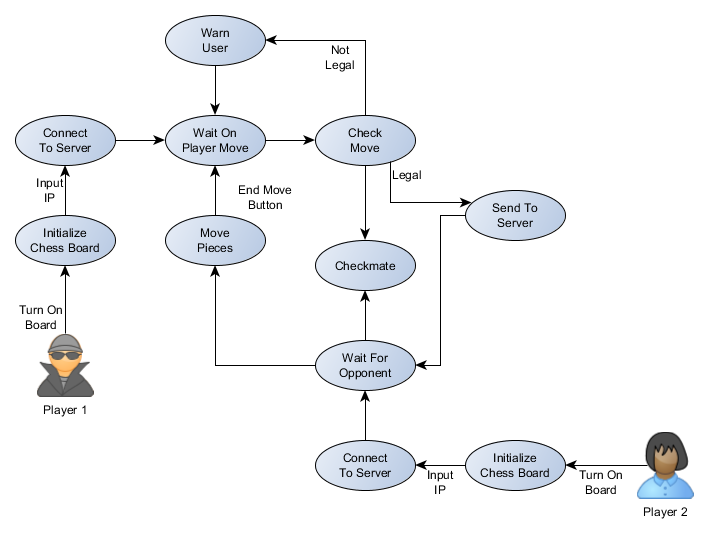
\includegraphics[scale=.5]{High_Level_State}}

\begin{center}
State diagram of the overall system, including the two users.
\end{center}

\vspace*{5mm}

\section*{Microcontroller}
\indent

Once the microcontroller is turned on, it will initialize anything it needs to. This includes the connecting the WiFi module, zeroing out the stepper motors, initializing the game state, connecting to the server to start a game, and prompting anything needed by the user or informing the user on the LCD. Once this has been completed by the micro controller the game can start. Assuming you are player one, it will start you off as white, which means you will go first. Otherwise you are player two and start as black. If you are player one the microcontroller will wait for you to move pieces by continuously scanning the reed switches and once a move has been detected, store that move and continue to scan. Once the user is finished moving the pieces, the user will confirm his move and the micro controller will check if that move is legal. If it is not it will revert back to detecting moves and storing the state. If it is legal and either a checkmate or stalemate, the microcontroller will prompt the server that the game has completed, and the current game will end there and restart a new one. If it is just a legal move, then it will send it to the WiFi. If the connection failed between the WiFi module and the server, the microcontroller will wait for reconnection and try to receive acknowledgment from the WiFi module that the information was sent. Upon success, the microcontroller will now wait for the opponents move. This is where player two’s state will start. When data is received the microcontroller will calculate exactly what move is done. If it a checkmate or stalemate your game will be over. If not it will then calculate how to move the pieces mechanically. The way the pieces will move is by moving along the edges of the squares and moving along the axises until it reaches the square destination and moves to the center of the square. This can be done because the pieces diameter will be less than half the width of the square. Then it will proceed to move the piece as necessary. If there are multiple pieces to move the microcontroller will repeat the steps done for the first piece. Upon completion of the pieces being moved, the stepper motors will recalibrate, then it will be your turn to play, detecting your moves. Thus it will cycle between turns until the game has been completed. The LCD will display information based on the current state.

\vspace*{5mm}

\centerline{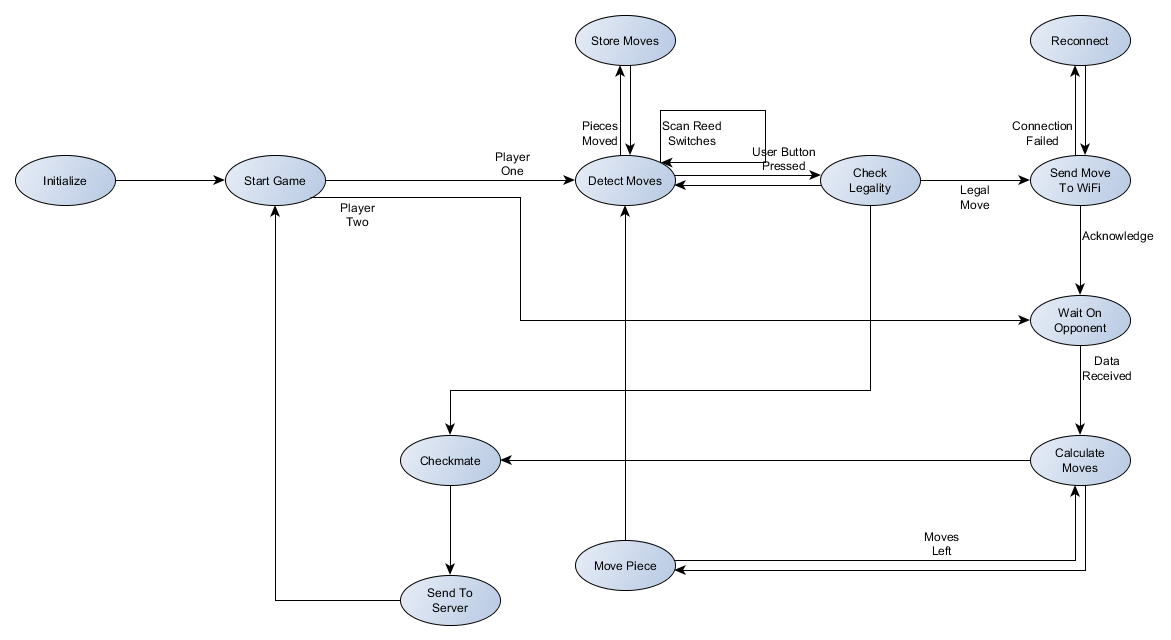
\includegraphics[scale=.4]{Microcontroller_State}}

\begin{center}
State diagram of the microcontroller system.
\end{center}

\vspace*{5mm}
	
\section*{WiFi Module}
\indent

The ESP8266 WiFi module state diagram starts in a state where it waits for a command. This command is through the UART serial bus from the microcontroller. At the start state of the module, it will receive the SSID and password for the WiFi network as well as the IP address for the server. Within this state, the module will be unable to perform activity involving a server querying until it is successful in connecting to a WiFi network. First a network is connected to using the SSID and password. If successful, acknowledgment is sent back to the module. An error will be sent if there is no successful connection. Once connected, using the IP address and the port number hardcoded in the firmware of the module, the module will connect to the server with acknowledgment of success or failure. The WiFi module has a tendency to lose connection to the network. Due to this problem, feedback is sent to the user specifying that disconnect has occurred. While the user is being informed, the program will begin to loop again, attempting to connect back to the network. Assuming all connections are in place and waiting for further action, in the event something is to be sent to the server, it will send the data, as always, with acknowledgment of the action. In the event something is requested from the server, the module will send a query request for data. Situations may arise that the server has nothing to send. The server will say that there is nothing to be sent. The data is received if there is something to be sent back from the server and then is sent back to the through the UART bus to the WiFi module to wait for the next command to be done.

\vspace*{5mm}

\centerline{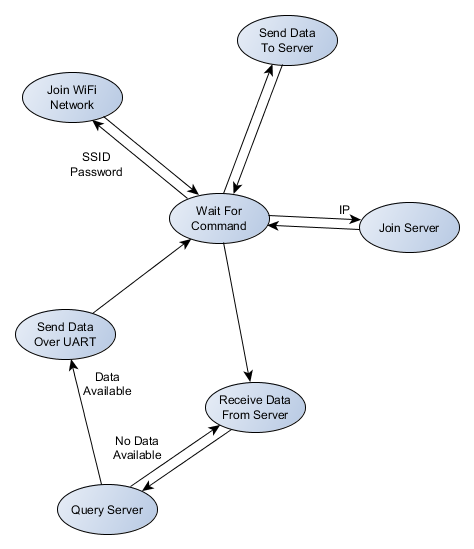
\includegraphics[scale=.5]{WiFi_Module_State}}

\begin{center}
State diagram of the WiFi module system.
\end{center}

\vspace*{5mm}

\section*{Server}
\indent

The server starts by initializing all the variables and structures it needs before players begin connecting to it. When one player connects, the server will have that player wait for an opponent to connect. Once two players are connected, the game will start.  

\indent  

During the game, a cycle will occur until the game ends by checkmate or by stalemate. The cycle begins with the server waiting on a move from player one. Once it receives a move from player one, the server will send that move to player two. The server then does the same for player two: it waits for player two to make a move, then it will send that move to player one. As stated above, this cycle repeats until one of the players makes a move that is checkmate (wherein the server will verify the checkmate and end the game), or by stalemate. Either player can declare a stalemate at any time, and the server will announce this decision to both players.  

\indent  

In the case of a player accidentally disconnecting from the server, the server will alert the still-connected player and allow 5 minutes for the dropped player to re-connect. If the player does not reconnect in the allotted time, the game will end in a draw. 

\indent

Thus, the server only keeps track of the players and their states for the duration of a game. It also handles raw data sent to it over the socket, but only for the duration of a single call to the server's handle function.

\indent

The server will be headless, that is to say it will only respond to the client boards that connect to it. It will also have only one operating mode for the time being - it will not automatically replay games that have been saved to the server because it does not store whole games.

\vspace*{5mm}

\centerline{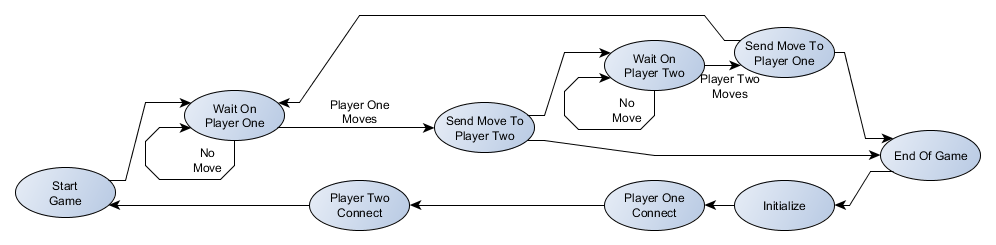
\includegraphics[scale=.5]{Server_State}}

\begin{center}
State diagram of the WiFi system.
\end{center}

\vspace*{5mm}

\section*{Hardware}
\indent

All the peripherals required to run the project, including LCD display, stepper motor drivers, electromagnet, and reed switch array, are interfaced to the microcontroller using general purpose input/output pins. These pins are software controllable, allowing the software to interface with the hardware. The microcontroller is connected to the WiFi module over a hardware UART bus, which differs from the GPIO's used to control the other peripherals but still allows software control of data between the microcontroller and WiFi module.

\section*{Schematic}
\indent

\vspace*{5mm}

\centerline{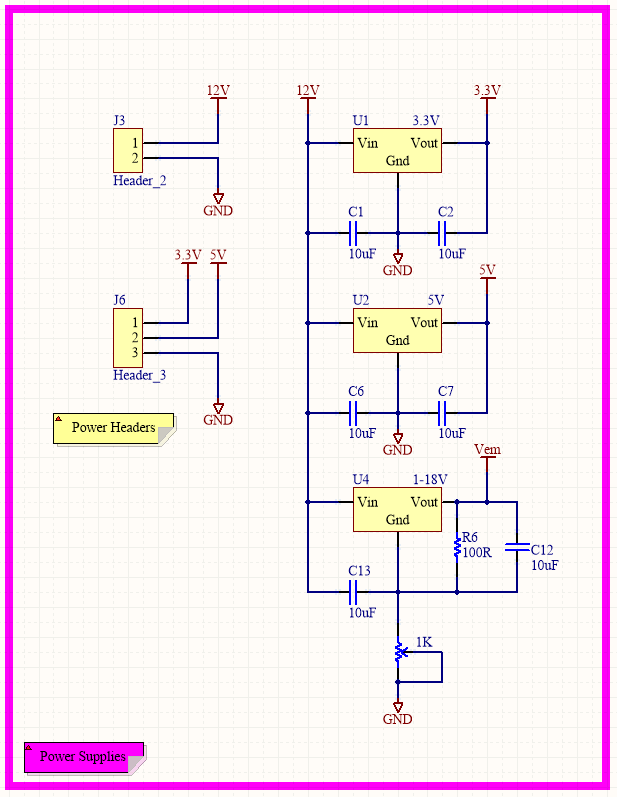
\includegraphics[scale=.75]{SchPowerSupply}}

\begin{center}
Schematic of the power supply of the embedded system. There is a header for the input power and a header for auxiliary output power. Three voltage regulators are used to provide the correct voltage levels of 5 volts for the microcontroller and peripherals, 3.3 volts for the WiFi module, and a variable 2-12 volts for the electromagnet.
\end{center}

\vspace*{5mm}

\vspace*{5mm}

\centerline{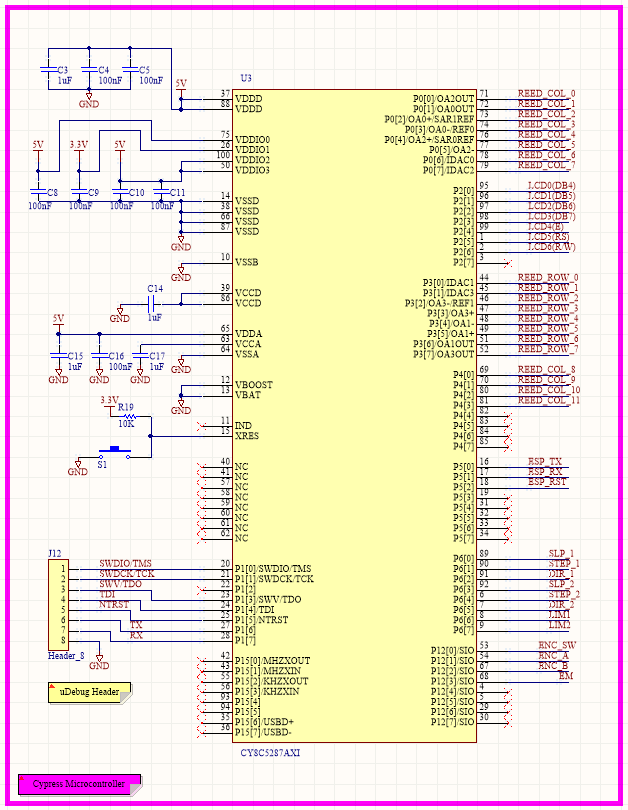
\includegraphics[scale=.75]{SchMicro}}

\begin{center}
Schematic of the microcontroller of the embedded system. It includes all the decoupling capacitors for the microcontroller power supply, as well as the reset switch and a header used for all the debug inputs and outputs to the microcontroller. The rest of the connections are to the peripherals used in the other sections.
\end{center}

\vspace*{5mm}

\vspace*{5mm}

\centerline{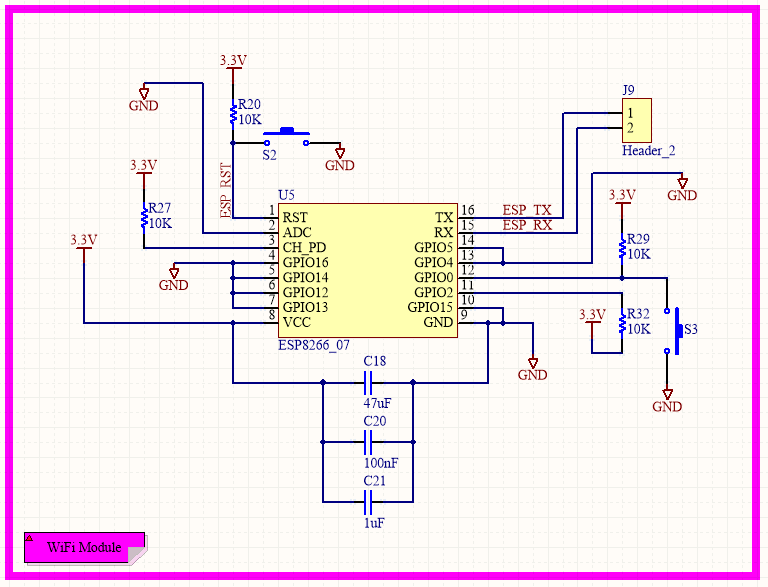
\includegraphics[scale=.75]{SchWiFi}}

\begin{center}
Schematic of the WiFi module of the embedded system. The WiFi module circuitry includes the decoupling capacitors for its power supply as well as a switch on the reset line and a switch to put the module into bootloader mode.
\end{center}

\vspace*{5mm}

\vspace*{5mm}

\centerline{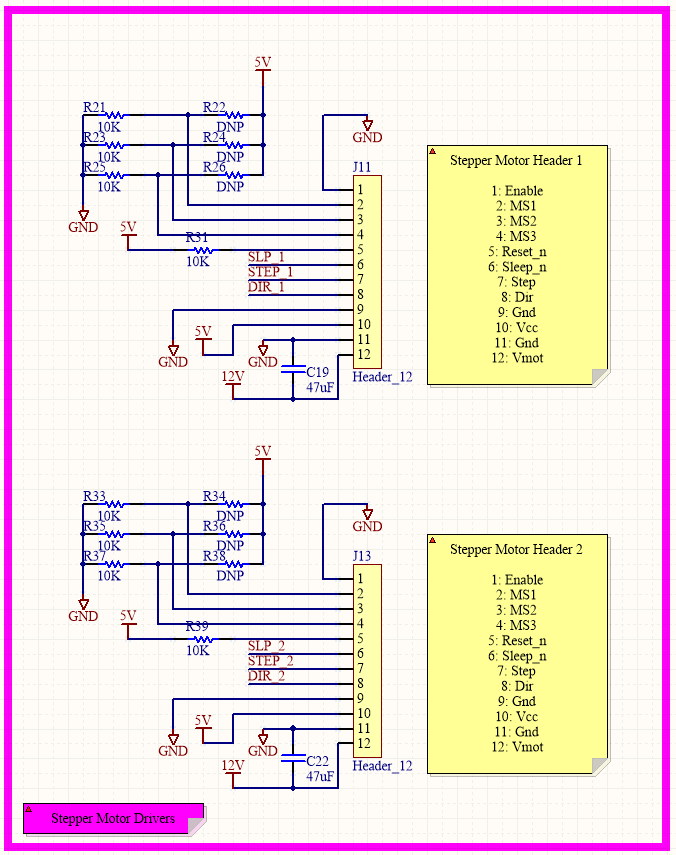
\includegraphics[scale=.75]{SchStepper}}

\begin{center}
Schematic of the stepper driver of the embedded system. This includes the connections to the motor supply voltage, the decoupling capacitors necessary and the resistors to set the microstepping value between 1x and 16x.
\end{center}

\vspace*{5mm}

\vspace*{5mm}

\centerline{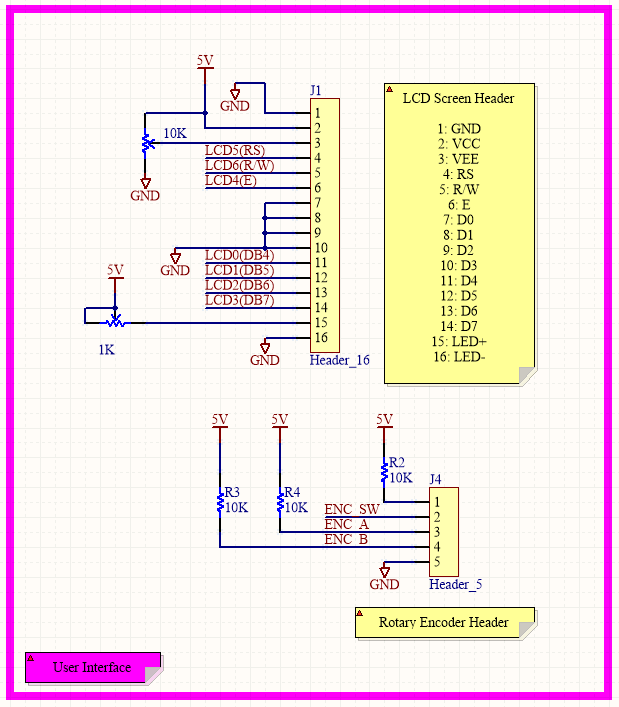
\includegraphics[scale=.75]{SchUI}}

\begin{center}
Schematic of the UI peripherals of the embedded system. This includes the header for the LCD character display and the header for the rotary encoder.
\end{center}

\vspace*{5mm}

\vspace*{5mm}

\centerline{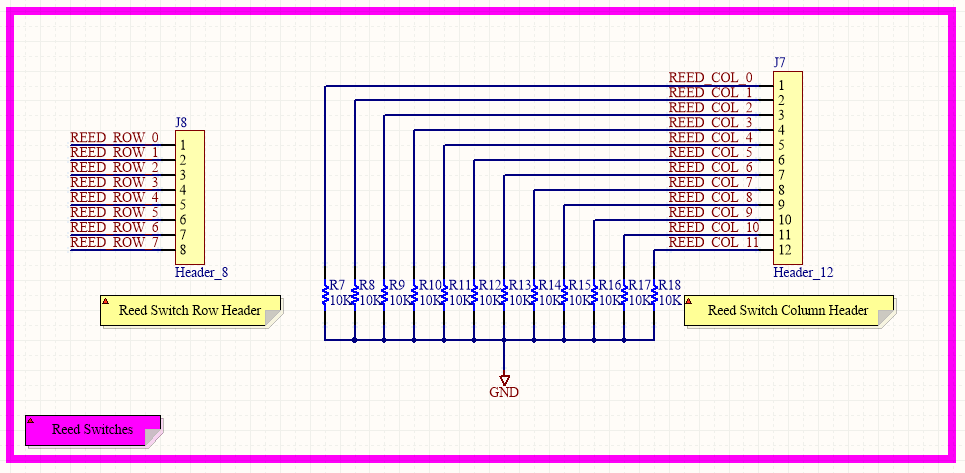
\includegraphics[scale=.75]{SchReed}}

\begin{center}
Schematic of the reed switch array interface of the embedded system. This consists of the headers for the array as well as the pulldown resistors for the column of the array.
\end{center}

\vspace*{5mm}

\vspace*{5mm}

\centerline{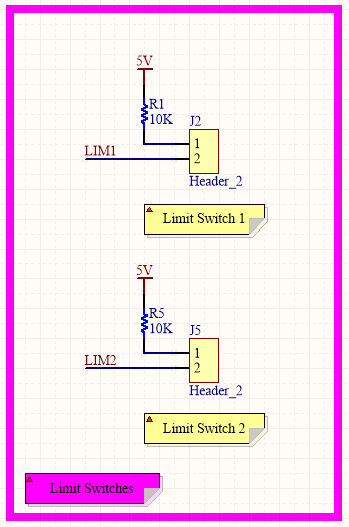
\includegraphics[scale=.75]{SchLim}}

\begin{center}
Schematic of the header connections to the limit switches.
\end{center}

\vspace*{5mm}

\vspace*{5mm}

\centerline{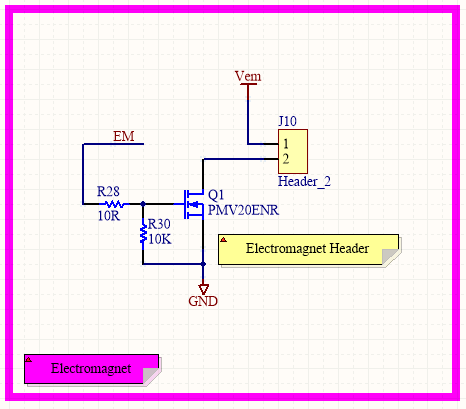
\includegraphics[scale=.75]{SchElectromagnet}}

\begin{center}
Schematic of the electromagnet circuitry of the embedded system. It uses a transistor to turn the electromagnet on and off by connecting and disconnecting it from the electromagnet power supply.
\end{center}

\vspace*{5mm}

\section*{Diagram Information}
\indent

For our project we determined that a UML state diagram would be the most fitting diagram. Because of the both sequential and cyclical nature of the game of chess it would be the most efficient way to represent our systems in graphical form. State diagrams also allow us to show how both players progress through their states at the same time as the other player, giving a sense of where a player would have to wait for his opponent.

\end{document}